\chapter{EXO-14-009}
\section{Introduction}
\label{sec:introduction}

Several physics models beyond the standard model (SM) predicts the
existence of vectorial  resonances with
masses above 1\TeVcc that decay into
a \PW\ or \cPZ\ vector boson, denoted as V boson,
  and a Higgs boson~\cite{Chatrchyan:2012ufa,higgsdiscoveryAtlas} .
In
proton-proton (pp) collisions at the energies reached at the Large Hadron
Collider (LHC), bosons emerging from such decays usually would have
sufficiently large momenta so that the hadronization products of their
 decays would merge into a single massive
jet~\cite{Gouzevitch:2013qca}. We present a search for events
containing jets of this kind in pp collisions at a
centre-of-mass energy of $\sqrt{s}=8$\TeVcc.  The data sample,
corresponding to an integrated luminosity of 19.7\fbinv, was collected
with the CMS detector at the LHC.

The signal of interest is a heavy vector resonance X, produced via the process
, ${\rm pp\to X\to H V}$, as in Figure~\ref{fig:Xdecays},  where
 the $V$ boson decay hadronically and the Higgs
 boson decay either to a $b$-quark pair or to
a pair of fully hadronic W bosons\footnote{As the Higgs
 boson branching ratio to Z bosons is about one-tenth of
its branching ratio to W bosons,
 we only consider the $H\to WW$ decay.}.

The resuts are interpreted in the following models of ${\rm \PWpr\to HW}$ and ${\rm Z'\to HZ}$ resonances.
The Composite-Higgs~\cite{Composite0,Composite1,Composite2} and Little Higgs models~\cite{Han:2003wu}
provide a direct solution to the hierarchy problem and predict many new particles,
including addtional gauge bosons, e.g. heavy $\PWpr$ or $Z'$ bosons.
Models of such type are generalized in the Heavy Vector Triplet (HVT) model~\cite{Pappadopulo:2014qza}.
Of particular interest for this search is the so called HVT scenario B model.
The
${\rm W^\prime}$ and ${\rm Z^\prime}$ decay to respective ${\rm WH}$ and ${\rm ZH}$ become dominant and almost degenarate
 with ${\rm W^\prime \rightarrow WZ}$,
such that these parameter points are not
 constrained so far from experiments (see Fig 3.2 in Ref.~\cite{Pappadopulo:2014qza}).
For $\PWpr$ with the SM coupling, the most stringent limits are reported in searches with
leptonic final states~\cite{CMSwprimePAPER2013,ATLASwprimePAPER}, and the current lower
limit on the $\PWpr$ mass is 2.9\TeVcc.
The limit varies by 0.1\TeVcc, depending on the chirality of the $\PWpr$ couplings.
Specific searches in the WZ final state have also 
been reported~\cite{CMSwprimeWZPAS,ATLASWWPAPER,ATLASwprimeWZPAS}
setting a lower limit of 1.1\TeVcc. 
For $Z'$ with the SM coupling, the most stringent limits are reported in searches with
leptonic final states~\cite{ATLASzprimePAPER,CMSzprimePAPER}, and the current lower
limit on the $Z'$ mass is 2.8\TeVcc.


\begin{figure}[ht!b]
\begin{center}
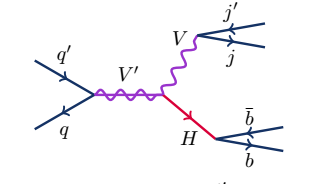
\includegraphics[width=0.49\textwidth]{EXO-14-009/figs/diagrambb.png}
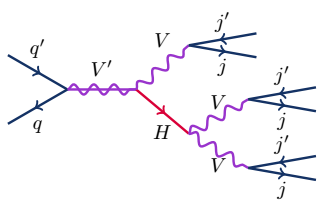
\includegraphics[width=0.49\textwidth]{EXO-14-009/figs/diagramww.png}
\end{center}
\caption{
X decays. 
%Signal shapes for Z' and W' signals at 1.0, 1.5, 2.0 and 2.5 TeV resonance.
% Z' are shown in solid lines,
%W' are shown in dashed lines, in H(bb)V decay(left) and H(ww)V decay(right).
}
\label{fig:Xdecays}
\end{figure}




The signal is characterized by a peak in the dijet invariant mass
distribution $m_\mathrm{jj}$ over a continuous background from SM
processes, comprised mainly of multijet events from quantum
chromodynamic (QCD) processes. The sensitivity to jets from Higgs decays to
$b$-quark pair is enhanced through subjets b-tagging~\cite{BTV-13-001}.
While jets from Higgs decays to hadronic W-pairs, and also jets from \PW\ or
\cPZ\ bosons are identified with jet-substructure
techniques~\cite{topwtag_pas,JME-13-006}.
Results for W' and Z', which decays to Higgs boson and one vector boson V, are
presented in this analysis.

This is the first search for the heavy resonances decaying to all 
hadronic HV final
states, as well as the first application of the highly boosted
$\Hww$ decays.


%This is the first search for the heavy resonances decaying to HV final
%state, as well as the first application of the highly boosted

This analysis proceeds via the following steps:
\begin{enumerate}
\item The search is performed in the dijet sample, using the same
      preselection as the standard search for resonances decaying to 
      dijets~\cite{cmsdijet, cmsdijet8TeV}.

\item We identify events with \PW\ or \cPZ: in each jet which is a candidate
  to originate from merging of V daughter jets:  
  \begin{itemize}
  \item we require a pruned jet mass cut, and
  \item an N-subjettiness cut preferring two-prong decays
  \end{itemize}
  (This is identical to EXO-12-024 \cite{CMS:2013fea}.)

\item We identify events with a highly boosted Higgs boson:
  \begin{itemize}
  \item we require a pruned jet mass cut, and
  \item two b tagged subjets, or 
  \item (when there are no two b tagged subjets) a N-subjettiness cut
    preferring four subjets
  \end{itemize}
  (The $\Hbb$ tagging is synchronized with our sister analysis, the Radion
  search to the HH final state~\cite{HH4b}.)

\item After the full event selection, a potential signal would be
  characterized as a peak in the dijet invariant mass, on top of a
  falling background distribution.  

\item We model the background distribution with a smoothly falling 
  analytical function.  (The functional form is identical
  to the one used in EXO-12-024.)

\item We form the joint likelihood of several dijet distributions
  of V tagged and H tagged jets.  We include both two types of
  Higgs tags, and also low-purity Higgs and V taggers.  The background
  estimate procedure is the same in all channels -- analytical
  prameterization -- but is performed separately for each channel.

\item Finally, we set the limits on the various simplified models
  for resonances decaying to HV final states.

\end{enumerate}
